\documentclass[tikz,border=5pt]{standalone}
\usepackage[UTF8]{ctex}
\usepackage{amsmath,amssymb}
\usetikzlibrary{arrows.meta,calc,angles,quotes,decorations.pathmorphing,patterns}
\definecolor{ink}{HTML}{243447}\definecolor{blue}{HTML}{2765A2}
\definecolor{green}{HTML}{3F7D5B}\definecolor{red}{HTML}{B74739}
\tikzset{body/.style={draw=ink,thick},vec/.style={draw=blue,thick,-{Latex}},guide/.style={gray!65,dashed},dim/.style={ink,{Latex}-{Latex}},line cap=round,line join=round}
\begin{document}

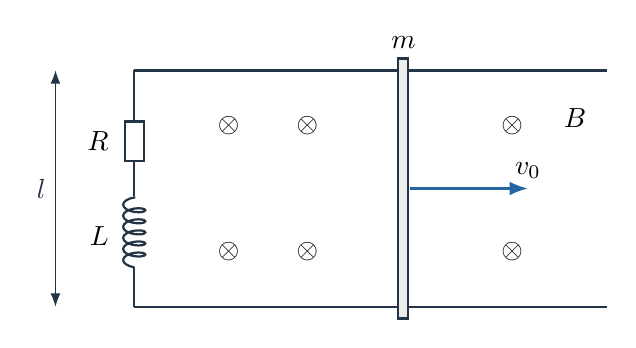
\begin{tikzpicture}
\draw[body](0,0)--(6,0);\draw[body](0,3)--(6,3);
\draw[body](0,0)--(0,.5);
\draw[body,decorate,decoration={coil,aspect=.4,segment length=4pt,amplitude=4pt}](0,.5)--(0,1.4);
\draw[body](0,1.4)--(0,1.85);\draw[body,fill=white](-.12,1.85)rectangle(.12,2.35);\draw[body](0,2.35)--(0,3);
\node[left]at(-.2,.9){$L$};\node[left]at(-.2,2.1){$R$};
\draw[body,fill=gray!15](3.35,-.15)rectangle(3.48,3.15);\node[above]at(3.42,3.15){$m$};
\draw[vec](3.5,1.5)--(5,1.5)node[above]{$v_0$};
\foreach \x in {1.2,2.2,4.8}\foreach \y in {.7,2.3}{\node at(\x,\y){$\otimes$};}
\node at(5.6,2.4){$B$};
\draw[dim](-1,0)--(-1,3)node[midway,left]{$l$};
\end{tikzpicture}
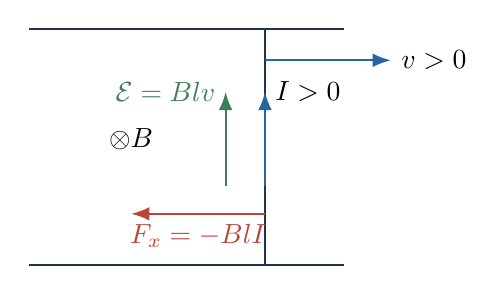
\begin{tikzpicture}
\draw[body](0,0)--(4,0);\draw[body](0,3)--(4,3);\draw[body,thick](3,0)--(3,3);
\draw[vec](3,1)--(3,2.2)node[right]{$I>0$};
\draw[vec](3,2.6)--(4.6,2.6)node[right]{$v>0$};
\draw[red,thick,-{Latex}](3,.65)--(1.3,.65)node[midway,below]{$F_x=-BlI$};
\node at(1.3,1.6){$\otimes B$};
\draw[green,thick,-{Latex}](2.5,1)--(2.5,2.2)node[left]{$\mathcal E=Blv$};
\end{tikzpicture}
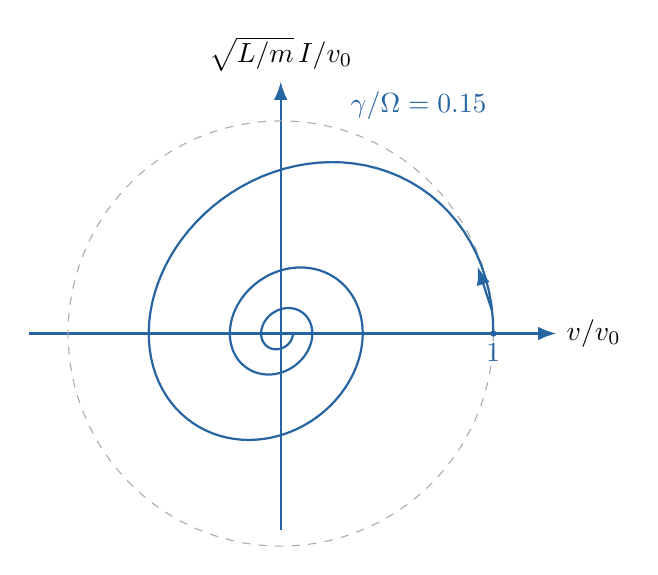
\begin{tikzpicture}
\draw[vec](-3.2,0)--(3.5,0)node[right]{$v/v_0$};
\draw[vec](0,-2.5)--(0,3.2)node[above]{$\sqrt{L/m}\,I/v_0$};
\draw[guide](0,0)circle(2.7);
\draw[blue,thick,domain=0:1100,samples=280,variable=\a]plot({2.7*exp(-.15*\a*pi/180)*(cos(.988686*\a)+.151716*sin(.988686*\a))},{2.730898*exp(-.15*\a*pi/180)*sin(.988686*\a)});
\fill[blue](2.7,0)circle(.04)node[below]{$1$};
\node[blue]at(1.75,2.9){$\gamma/\Omega=0.15$};
\draw[vec](2.68,.3)--(2.5,.85);
\end{tikzpicture}
\begin{tikzpicture}
\draw[vec](0,0)--(7.1,0)node[right]{$\Omega t$};\draw[vec](0,0)--(0,3.6)node[above]{$E/E_0$};
\draw[blue,thick,domain=0:6.5,samples=160]plot(\x,{3*exp(-.3*\x)*(pow(cos(.988686*\x*180/pi)+.151716*sin(.988686*\x*180/pi),2)+pow(1.011443*sin(.988686*\x*180/pi),2))});
\draw[green,thick,domain=0:6.5,samples=160]plot(\x,{3*exp(-.3*\x)*pow(cos(.988686*\x*180/pi)+.151716*sin(.988686*\x*180/pi),2)});
\draw[red,dashed,thick,domain=0:6.5,samples=160]plot(\x,{3*exp(-.3*\x)*pow(1.011443*sin(.988686*\x*180/pi),2)});
\node[left]at(0,3){$1$};
\node[blue]at(4.6,2.75){总能量};
\node[green]at(4.6,2.3){机械能};
\node[red]at(4.6,1.85){磁场能};
\end{tikzpicture}
\end{document}
